\documentclass[a4paper]{article}

\usepackage[text={18.6cm, 26.0cm}, centering]{geometry}

\usepackage[czech, provide=*]{babel}
\usepackage[utf8]{inputenc}
\usepackage[T1]{fontenc}
\usepackage{color}
\usepackage{graphicx}
\usepackage{alltt} % \verb
\usepackage[]{hyperref} % odkazy
\usepackage{tikz}


\usepackage[table]{xcolor}

\newcommand{\precTable}{
\begin{table}[h!]
\centering

% Resizing the table to fit the text width because it is very wide
%\resizebox{\textwidth}{!}{%
\begin{tabular}{|c|c|c|c|c|c|c|c|c|c|c|c|c|c|c|c|c|c|c|c|c|}
\hline
\cellcolor{gray} & \textbf{$+$} & \textbf{$-$} & \textbf{$*$} & \textbf{$/$} & \textbf{$>$} & \textbf{$<$} & \textbf{$>=$} & \textbf{$<=$} & \textbf{$==$} & \textbf{$!=$} & \textbf{$\&\&$} & \textbf{$||$} & \textbf{$id$} & \textbf{$($} & \textbf{$)$} & \textbf{$is$} & \textbf{$?$} & \textbf{$:$} & \textbf{$!$} & \textbf{$\$$} \\ \hline
\textbf{$+$} & $>$ & $>$ & $<$ & $<$ & $>$ & $>$ & $>$ & $>$ & $>$ & $>$ & $>$ & $>$ & $<$ & $<$ & $>$ & $>$ & $>$ & $>$ & $<$ & $>$ \\ \hline
\textbf{$-$} & $>$ & $>$ & $<$ & $<$ & $>$ & $>$ & $>$ & $>$ & $>$ & $>$ & $>$ & $>$ & $<$ & $<$ & $>$ & $>$ & $>$ & $>$ & $<$ & $>$ \\ \hline
\textbf{$*$} & $>$ & $>$ & $>$ & $>$ & $>$ & $>$ & $>$ & $>$ & $>$ & $>$ & $>$ & $>$ & $<$ & $<$ & $>$ & $>$ & $>$ & $>$ & $<$ & $>$ \\ \hline
\textbf{$/$} & $>$ & $>$ & $>$ & $>$ & $>$ & $>$ & $>$ & $>$ & $>$ & $>$ & $>$ & $>$ & $<$ & $<$ & $>$ & $>$ & $>$ & $>$ & $<$ & $>$ \\ \hline
\textbf{$>$} & $<$ & $<$ & $<$ & $<$ & $>$ & $>$ & $>$ & $>$ & $>$ & $>$ & $>$ & $>$ & $<$ & $<$ & $>$ & $>$ & $>$ & $>$ & $<$ & $>$ \\ \hline
\textbf{$<$} & $<$ & $<$ & $<$ & $<$ & $>$ & $>$ & $>$ & $>$ & $>$ & $>$ & $>$ & $>$ & $<$ & $<$ & $>$ & $>$ & $>$ & $>$ & $<$ & $>$ \\ \hline
\textbf{$>=$} & $<$ & $<$ & $<$ & $<$ & $>$ & $>$ & $>$ & $>$ & $>$ & $>$ & $>$ & $>$ & $<$ & $<$ & $>$ & $>$ & $>$ & $>$ & $<$ & $>$ \\ \hline
\textbf{$<=$} & $<$ & $<$ & $<$ & $<$ & $>$ & $>$ & $>$ & $>$ & $>$ & $>$ & $>$ & $>$ & $<$ & $<$ & $>$ & $>$ & $>$ & $>$ & $<$ & $>$ \\ \hline
\textbf{$==$} & $<$ & $<$ & $<$ & $<$ & $<$ & $<$ & $<$ & $<$ & $>$ & $>$ & $>$ & $>$ & $<$ & $<$ & $>$ & $<$ & $>$ & $>$ & $<$ & $>$ \\ \hline
\textbf{$!=$} & $<$ & $<$ & $<$ & $<$ & $<$ & $<$ & $<$ & $<$ & $>$ & $>$ & $>$ & $>$ & $<$ & $<$ & $>$ & $<$ & $>$ & $>$ & $<$ & $>$ \\ \hline
\textbf{$\&\&$} & $<$ & $<$ & $<$ & $<$ & $<$ & $<$ & $<$ & $<$ & $<$ & $<$ & $>$ & $>$ & $<$ & $<$ & $>$ & $<$ & $>$ & $>$ & $<$ & $>$ \\ \hline
\textbf{$||$} & $<$ & $<$ & $<$ & $<$ & $<$ & $<$ & $<$ & $<$ & $<$ & $<$ & $<$ & $>$ & $<$ & $<$ & $>$ & $<$ & $>$ & $>$ & $<$ & $>$ \\ \hline
\textbf{$id$} & $>$ & $>$ & $>$ & $>$ & $>$ & $>$ & $>$ & $>$ & $>$ & $>$ & $>$ & $>$ & \cellcolor{red} & \cellcolor{red} & $>$ & $>$ & $>$ & $>$ & $>$ & $>$ \\ \hline
\textbf{$($} & $<$ & $<$ & $<$ & $<$ & $<$ & $<$ & $<$ & $<$ & $<$ & $<$ & $<$ & $<$ & $<$ & $<$ & $=$ & $<$ & $<$ & $<$ & $<$ & \cellcolor{red} \\ \hline
\textbf{$)$} & $>$ & $>$ & $>$ & $>$ & $>$ & $>$ & $>$ & $>$ & $>$ & $>$ & $>$ & $>$ & \cellcolor{red} & \cellcolor{red} & $>$ & $>$ & $>$ & $>$ & \cellcolor{red} & $>$ \\ \hline
\textbf{$is$} & $<$ & $<$ & $<$ & $<$ & $<$ & $<$ & $<$ & $<$ & $>$ & $>$ & $>$ & $>$ & $<$ & $<$ & $>$ & $>$ & $>$ & $>$ & $<$ & $>$ \\ \hline
\textbf{$?$} & $<$ & $<$ & $<$ & $<$ & $<$ & $<$ & $<$ & $<$ & $<$ & $<$ & $<$ & $<$ & $<$ & $<$ & $>$ & $<$ & \cellcolor{red} & $=$ & $<$ & $>$ \\ \hline
\textbf{$:$} & $<$ & $<$ & $<$ & $<$ & $<$ & $<$ & $<$ & $<$ & $<$ & $<$ & $<$ & $<$ & $<$ & $<$ & $>$ & $<$ & $<$ & \cellcolor{red} & $<$ & $>$ \\ \hline
\textbf{$!$} & $>$ & $>$ & $>$ & $>$ & $>$ & $>$ & $>$ & $>$ & $>$ & $>$ & $>$ & $>$ & $<$ & $<$ & $>$ & $<$ & $>$ & $>$ & $<$ & $>$ \\ \hline
\textbf{$\$$} & $<$ & $<$ & $<$ & $<$ & $<$ & $<$ & $<$ & $<$ & $<$ & $<$ & $<$ & $<$ & $<$ & $<$ & \cellcolor{red} & $<$ & $<$ & \cellcolor{red} & $<$ & \cellcolor{red} \\ \hline
\end{tabular}%
%}
\caption{Precedenční tabulka}
\end{table}}

\newcommand{\llTable}{
\begin{table}[h!]
\centering

% Resizing the table to fit the text width
\resizebox{0.95\textwidth}{!}{%
\begin{tabular}{|c|c|c|c|c|c|c|c|c|c|c|c|c|c|c|c|c|c|c|}
\hline
\cellcolor{gray} & \textbf{\texttt{import}} & \textbf{\texttt{class}} & 
\textbf{\texttt{static}} & \textbf{\texttt{id}} & \textbf{\texttt{\_\_id}} & \textbf{\texttt{var}} & 
\textbf{\texttt{(}} & \textbf{\texttt{)}} & \textbf{\texttt{if}} & \textbf{\texttt{else}} & 
\textbf{\texttt{while}} & \textbf{\texttt{return}} & \textbf{\texttt{\{}} & \textbf{\texttt{\}}} & \textbf{\texttt{=}} & \textbf{\texttt{,}} & \textbf{\texttt{<EOL>}} & \textbf{ostatní} \\ \hline
\textbf{<program>} & 1 &&&&&&&&&&&&&&&&&  \\ \hline
\textbf{<prologue>} & 2 &&&&&&&&&&&&&&&&&  \\ \hline
\textbf{<class\_program>} && 3 &&&&&&&&&&&&&&&&  \\ \hline
\textbf{<class\_body>} &&& 5 &&&&&&&&&&& 4 &&&&  \\ \hline
\textbf{<statics>} &&&&&&& 8 &&&&&& 7 && 6 &&&  \\ \hline
\textbf{<params>} &&&& 10 &&&& 9 &&&&&&&&&&  \\ \hline
\textbf{<params\_c>} &&&&&&&&12&&&&&&&& 11 &&  \\ \hline
\textbf{<body>} &&&& 15 & 13 & 14 &&& 16 && 17 & 18 & 21 &&&&& 20  \\ \hline
\textbf{<assign>} &&&&&&&&&&&&&&& 23 && 22 &  \\ \hline
\textbf{<els>} &&&&&&&&&& 25 &&&&&&& 24 &  \\ \hline
\textbf{<elif>} &&&&&&&&& 27 &&&& 26 &&&&&  \\ \hline
\textbf{<return\_stat>} &&&&&&&&&&&&&&&&& 28 & 29 \\ \hline
\end{tabular}%
}
\caption{LL tabulka}
\end{table}
}


\newcommand{\grammar}{
\begin{enumerate}
    \item <program> $\rightarrow$ <prologue> <EOL> <class\_program>
    \item <prologue> $\rightarrow$ \textbf{import "ifj25" for Ifj}
    \item <class\_program> $\rightarrow$ \textbf{class Program \{ <EOL>} <class\_body> \textbf{\}}
    \item <class\_body> $\rightarrow$ $\varepsilon$
    \item <class\_body> $\rightarrow$ \textbf{static id} <statics>
    \item <statics> $\rightarrow$ = \textbf{( id ) \{ <EOL>}  <body> \textbf{\} <EOL>} <class\_body>
    \item <statics> $\rightarrow$ \textbf{\{ <EOL>} <body> \textbf{\} <EOL>} <class\_body>
    \item <statics> $\rightarrow$ \textbf{(} <params> \textbf{) \{ <EOL>} <body> \textbf{\} <EOL>} <class\_body>
    \item <params> $\rightarrow$ $\varepsilon$
    \item <params> $\rightarrow$ \textbf{id} <params\_c>
    \item <params\_c> $\rightarrow$ \textbf{, id} <params>
    \item <params\_c> $\rightarrow$ $\varepsilon$
    \item <body> $\rightarrow$ \textbf{\_\_id} <assign> <body>
    \item <body> $\rightarrow$ \textbf{var id} <assign> <body>
    \item <body> $\rightarrow$ \textbf{id =} <expr> \textbf{<EOL>} <body>
    \item <body> $\rightarrow$ \textbf{if (} <expr> \textbf{) \{ <EOL>} <body> \textbf{\}} <els>
    \item <body> $\rightarrow$ \textbf{while (} <expr> \textbf{) \{ <EOL>} <body> \textbf{\} <EOL>}
    \item <body> $\rightarrow$ \textbf{return} <return\_stat>
    \item <body> $\rightarrow$ $\varepsilon$
    \item <body> $\rightarrow$ <expr> \textbf{<EOL>}
    \item <body> $\rightarrow$ \textbf{\{ <EOL>} <body> \textbf{\} <EOL>}
    \item <assign> $\rightarrow$ \textbf{<EOL>}
    \item <assign> $\rightarrow$ \textbf{=} <expr> \textbf{<EOL>}
    \item <els> $\rightarrow$ \textbf{<EOL>}
    \item <els> $\rightarrow$ \textbf{else} <elif>
    \item <elif> $\rightarrow$ \textbf{\{ <EOL>} <body> \textbf{\} <EOL>}
    \item <elif> $\rightarrow$ \textbf{if (} <expr> \textbf{) \{ <EOL>} <body> \textbf{\}} <els>
    \item <return\_stat> $\rightarrow$ \textbf{<EOL>}
    \item <return\_stat> $\rightarrow$ <expr> \textbf{<EOL>}
\end{enumerate}
}
% Ceske uvozovky
\providecommand{\uv}[1]{\quotedblbase #1\textquotedblleft}

\begin{document}
    \begin{titlepage}
        \begin{center}
            \textsc{\Huge{}Vysoké učení technické v Brně\\[0.5em]}
            \textsc{\huge Fakulta informačních technologií}\\
            \vspace{\stretch{0.382}}
            { \huge Wren překladač\,--\,dokumentace\\[0.5em]
                IFJ/IAL 2025 }\\[0.5em]
                Tým xsebesm00, varianta TRP-izp\\
            \vspace{\stretch{0.618}}
        \end{center}
        { \phantom{a}\hfill FUNEXP\\
          \phantom{a}\hfill EXTSTAT\\
          Vojtěch Borýsek (xborysv00)\,--\, 33\% \hfill EXTFUN\\
          Šimon Halas (xhalass00)\,--\, 00\% \hfill BOOLTHEN\\
          Tomáš Hanák (xhanakt00)\,--\, 33\% \hfill OPERATORS\\
          Michal Šebesta (xsebesm00)\,--\, 34\%, vedoucí \hfill STATICAN\\
          }
    \end{titlepage}
    \tableofcontents
    \newpage
    \section{Přehled}
        \begin{figure}[ht]
            \centering
            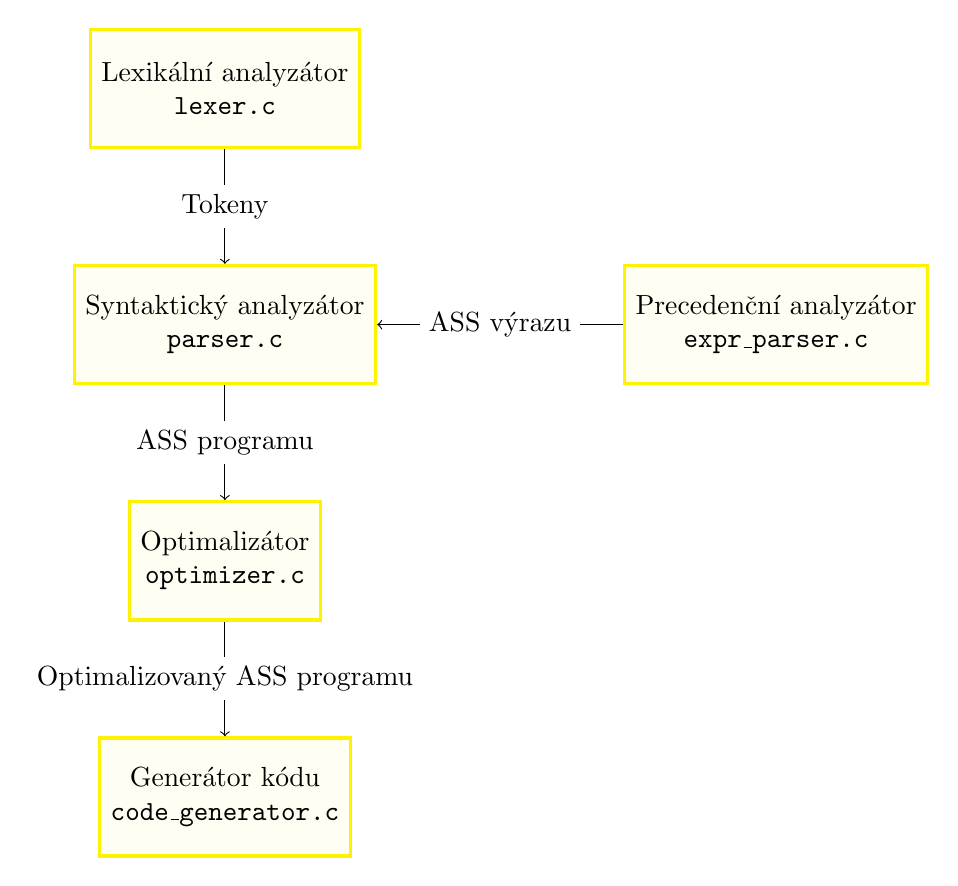
\begin{tikzpicture}[
                    every node/.style={fill=white},
                    block/.style={rectangle, draw=yellow, fill=yellow!5, very thick, minimum size=15mm, inner sep=4pt,draw},
                    node distance=3cm,
                    align=center,
                ]
                \node[block] (lexer) {Lexikální analyzátor\\ \texttt{lexer.c}};
                \node[block] (parser) [below of=lexer] {Syntaktický analyzátor\\ \texttt{parser.c}};
                \node[block] (expr) [right of=parser, xshift=4cm]{Precedenční analyzátor\\ \texttt{expr\_parser.c}};
                \node[block] (optimizer) [below of=parser] {Optimalizátor\\ \texttt{optimizer.c}};
                \node[block] (codegen) [below of=optimizer] {Generátor kódu\\ \texttt{code\_generator.c}};

                \draw[->] (lexer.south) -- node {Tokeny} (parser.north);
                \draw[->] (expr.west) -- node {ASS výrazu} (parser.east);
                \draw[->] (parser.south) -- node {ASS programu} (optimizer.north);
                \draw[->] (optimizer.south) -- node {Optimalizovaný ASS programu} (codegen.north);
            \end{tikzpicture}
            \caption{Diagram komponent překladače}
            \label{fig:compiler-diagram}
        \end{figure}
        Překlad začíná inicializací lexikálního analyzátoru. Ten je následně předán syntaktickému analyzátoru,
        který jej volá v případě potřeby tokenu. Pokud syntaktický analyzátor potřebuje načíst výraz, volá precedenční
        analyzátor. V rámci syntaktického analyzátoru se rovnou také provádí sémantické akce,
        jako kontrola typů výrazů, nebo kontrola deklarace proměnných. Výsledek ukládá do abstraktního
        syntaktického stromu (ASS).

        Jakmile je celý program převeden na ASS a sémanticky zkontrolován, je tento strom předán do optimalizátoru, který strom zoptimalizuje.
        Optimalizovaný strom je následně předán generátoru kódu, který z něj vytvoří cílový kód, čímž překlad končí.


    \section{Lexikální analýza}
        Lexikální analyzátor čte vstupní program a rozděluje ho na jednotlivé tokeny. Je volán syntaktickým analyzátorem,
        kontkrétně metodou \texttt{lexer\_get\_token()}. K dispozici je také funkce \texttt{lexer\_unget\_token()}, která
        syntaktickému analyzátoru umožňuje token vrátit a načíst ho později, což se hodí v situacích,
        kde další pravidlo není jasné a může být potřeba token vrátit jiné proceduře.


        \begin{figure}[ht]
            \centering
            \includegraphics{fsm.pdf}
            \caption{Diagram konečného automatu}
            \label{fig:fsm}
        \end{figure}

        Lexikální analyzátor je implementován jako konečný stavový automat (\ref{fig:fsm}). Většinu typů tokenů jsme schopni
        pokrýt pouze automatem. U některých typů ale musíme vyzužít něco navíc. Lexikální analyzátor má k
        dispozici dva znakové buffery a jeden čítač, které využívá k načtení následujících typů tokenů.

        \subsection{Číselné literály}
            V momentě kdy automat přejde do stavu, kde se začíná zpracovávat číselný literál, začne
            vstupní znaky psát do \texttt{buf1}. Jakmile narazíme na konec literálu, výsledný řetězec je
            převeden na \texttt{double} pomocí funkce \texttt{strtod()} nebo \texttt{hex2int}.

        \subsection{Řetězcové literály}
            Klasické řetězcové literály se zapisují do \texttt{buf1} a výsledek je na konci vrácen uvnitř
            tokenu.

            Víceřádkové řetězcové literály jsou složitější. Znaky se nejprve čtou do \texttt{buf2}
            dokud se nenarazí na znak nového řádku. V ten moment se obsah \texttt{buf2} přidá na konec
            \texttt{buf1}, pokud řádek v \texttt{buf2} není první nebo poslední. V tom případě se do
            \texttt{buf1} nepřidá pokud je prázdný nebo obsahuje pouze bílé znaky.
        \subsection{Víceřádkové komentáře}
            Víceřádkové komentáře mohou být zanořeny, takže lexikální analyzátor potřebuje čítač
            zanoření. Při uzavření víceřádkového komentáře se podle stavu čítače přejde do stavu
            uvnitř komentáře nebo mimo komentář.

        \subsection{Identifikátory a klíčová slova}
            Automat nijak nerozlišuje klíčová slova. Z jeho pohledu načte identifikátor, který
            čte do \texttt{buf1}. Než je token identifikátoru vrácen, lexikální analyzátor se
            podívá do tabulky klíčových slov a pokud v ní načtený text najde, vrátí místo tokenu
            identifikátoru token správného klíčového slova.

        Zbytek tokenů můžeme načíst pouze pomocí konečného automatu bez dalších neformalit.

        Nové řádky se berou jako token, a jejich správné umístění řeší syntaktická analýza.

        Lexikální analyzátor také přijímá tokeny pro zadání rozsahu do příkazu \texttt{for}, ale
        celé rozšíření nakonec implementováno nebylo.

    \section{Syntaktický analýza}
        TODO
        \grammar
        \llTable
    \subsection{Tabulka symbolů}
        TODO
    \subsection{Sémantická analýza}
        TODO
    \subsection{Zpracování výrazů}
        TODO
        \precTable
    \subsection{Abstraktní syntaktický strom}
        TODO

    \section{Optimalizátor}
        Optimalizátor provádí optimalizaci abstraktního syntaktického stromu před jeho předáním generátoru kódu.
        Prochází celý ASS rekurzivně a vyhodnocuje výrazy, které lze vypočítat již v době překladu, čímž
        snižuje složitost výsledného kódu a zvyšuje rychlost běhu programu.

        \subsection{Vyhodnocování konstantních výrazů}
        Optimalizátor vyhodnocuje výrazy, jejichž všechny operandy jsou známé v době překladu.
        Příklad aritmetické operace:
        \begin{alltt}
2 + 3  \(\rightarrow\)  5
        \end{alltt}

        \subsection{Vyhodnocování vestavěných funkcí}
        Optimalizátor dokáže vyhodnotit volání vestavěných funkcí s konstantními parametry.
        Příklad:
        \begin{alltt}
Ifj.length("hello")  \(\rightarrow\)  5.0
        \end{alltt}

        \subsection{Propagace konstant}
        Optimalizátor sleduje hodnoty proměnných a využívá je k další optimalizaci. 
        Pokud je hodnota proměnné známá, nahradí její použití přímo hodnotou:
        \begin{alltt}
var x = 5
var y = x + 3    // x je známé \(\rightarrow\) y = 5 + 3 \(\rightarrow\) y = 8
var z = y * 2    // y je známé \(\rightarrow\) z = 8 * 2 \(\rightarrow\) z = 16
        \end{alltt}

        \subsection{Ošetření vedlejších efektů}
        Optimalizátor musí správně zacházet s operacemi, které mohou mít vedlejší efekty.
        Při volání funkcí, getterů a setterů se maží všechny známé hodnoty globálních proměnných,
        protože tyto operace mohou proměnné modifikovat. V podmínkách a cyklech se rovněž maží
        známé hodnoty, protože není jisté, která větev se vykoná nebo kolikrát se cyklus opakuje.

        Vstupním bodem je funkce \texttt{optimize\_ast()}, která inicializuje optimalizaci celého programu.

    \section{Generátor kódu}
        Generátor kódu přijímá ASS a generuje z něj cílový program v IFJcode25. Vstupní metoda generátoru
        je \texttt{generate\_code()}. Generování následně probíhá následovně:
        \begin{enumerate}
            \item Podle globální tabulky symbolů se vygenerují deklarace globálních proměnných a jejich
                inicializace na \texttt{nil}.
            \item Deklaruje se 7 interních překladačových globálních proměnných, se kterými dále pracujeme při
                vyhodnocování výrazů.
            \item Vygenerujeme kód, která zavolá funkci \texttt{main()} a po návratu ukončí program s kódem 0.
            \item Generujeme jednotlivé funkce.
        \end{enumerate}
        \subsection{Generování funkcí}
            Na začátku vygenerujeme pro funkci návěští a vytvoříme nový rámec proměnných. Název funkce je
            zapsán ve formátu \texttt{fun\$x} kde \texttt{fun} je název funkce a \texttt{x} je počet jejích
            parametrů. Následně podle lokální tabulky symbolů vygenerujeme deklarace všech lokálních proměnných.

            Dále do lokálních proměnných reprezentující parametry funkce vložíme argumenty, které se podle
            konvence volání nachází na zásobníku hodnot. Na vrcholu zásobníku vždy bude poslední argument,
            volaný je tedy popuje v obráceném pořadí.

            Pak už se generuje tělo funkce.

            Na konci se vygeneruje implicitní příkaz \texttt{return}, spolu s příkazem \texttt{POPFRAME} a
            vložením hodnoty \texttt{nil}, implicitní návratové hodnoty, na zásobník.

        \subsection{Generování příkazů}
            Pro každý možný příkaz v ASS existuje procedura, která pro tento příkaz vygeneruje cílový kód.
            \begin{itemize}
                \item \texttt{ST\_BLOCK}: Iteruje přes všechny příkazy a uvnitř bloku a generuje pro ně kód.
                \item \texttt{ST\_IF}: Vygeneruje vyhodnocení pravdivosti výrazu a podle něj skočí na správné návěští.
                \item \texttt{ST\_WHILE}: Vygeneruje vyhodnocení pravdivosti výrazu a podle něj cyklus opustí nebo v něm pokračuje. Na konci těla cyklu se skočí zpět na vyhodnocení pravdivosti.
                \item \texttt{ST\_RETURN}: Vloží na vrchol zásobníku \texttt{nil} nebo vyhodnotí vracený výraz pokud je dán. Následně vygeneruje příkazy \texttt{POPFRAME} a \texttt{RETURN}.
                \item \texttt{ST\_LOCAL\_VAR}: Pokud není dán výraz, který se má přiřadit, vloží se do proměnné \texttt{nil}. Pokud výraz dán je, vyhodnotí se a jeho hodnota se uloží do proměnné
                    z vrochu zásobníku.
                \item \texttt{ST\_GLOBAL\_VAR}: Vyhodnotí se přiřazovaný výraz a jeho hodnota se uloží do proměnné.
                \item \texttt{ST\_SETTER\_CALL}: Vyhodnotí se přiřazovaný výraz a zavolá se setter.
                \item \texttt{ST\_EXPRESSION}: Samostojící výraz se vyhodnotí a jeho hodnota se z vrcholu zásobníku zahodí.
            \end{itemize}
            \subsubsection{Optimalizace}
                Pokud přiřazujeme do proměnné výraz se známou hodnotou, místo toho, abychom ji pushnuli a následně popnuli,
                vygenerujeme rovnou instrukci \texttt{MOVE}. Například u \texttt{a = 5 + 5} se vygeneruje \texttt{MOVE LF@a?0 float@0x1.4p+3}
                namísto
                \begin{alltt}
PUSHS float@0x1.4p+3
POPS LF@a!0 \end{alltt}

                Při vyhodnocování pravdivostní hodnoty můžeme zjistit, že některé větve není potřeba generovat.
                Tuto informaci vrací funkce, které vyhodnocení pravdivosti generuje, a můžeme podle ní některé
                větve vypustit. Například u
                \begin{alltt}
if (null) \{
    ...
\} else \{
    ...
\} \end{alltt}
                není potřeba generovat větev \uv{pravda.}
        \subsection{Generování výrazů}
            Vyhodnocování výrazů probíhá na zásobníku. Nejdříve se rekurzivně vyhodnotí každý podvýraz a jejich
            hodnoty zůstanou na vrcholu zásobníku. Následně se provede jejich typová kontrola a výraz se vyhodnotí.

            Se všemi čísly se ve výsledném programu pracuje jako s \texttt{float}y. Ke konverzi na \texttt{int} dochází
            pouze v případě kde je celočíselnost potřeba, např. při operátoru iterace řetězce nebo v některých
            vestavěných funkcích.

            Jako výrazy se berou také vestavěné funkce. Tyto funkce se vyhodnocují na místě bez jakéhokoliv volání.

            Také normální funkce a gettery se berou jako výrazy a jejich vyhodnocování probíhá následovně:
            \begin{enumerate}
                \item Vyhodnotí se všechny podvýrazy reprezentující argumenty. Jejich hodnoty zůstanou na vrcholu zásobníku.
                \item Zavolá se funkce, která argumenty z vrcholu zásobníku převezme.
                \item Funkce nechá návratovou hodnotu na vrcholu zásobníku, kde si ji převezme nadvýraz.
            \end{enumerate}

            \subsubsection{Optimalizace}
                U každého výrazu mohou být ze sémantické analýzy uvedeny informace o typu výrazu a případně
                i jeho hodnota, pokud ji optimalizátor dokázal vypočítat. Pokud jsou tyto informace k dispozici,
                můžeme si někdy odpustit generování typové kontroly a někdy i samotného vyhodnocení výrazu.

                Například u \texttt{a = ("ahoj" * 2) + \_\_unknown} optimalizátor ví, že první podvýraz nabývá
                hodnoty \texttt{"ahojahoj"}, takže nic nevyhodnocujeme a jen vložíme vypočtenou hodnotu na zásobník. Při vyhodnocování
                operátoru \texttt{+} pak nemusíme kontrolovat typ levého podvýrazu, protože je ze sémantické analýzy
                jasný. Také jistě víme, že zde operátor \texttt{+} označuje konkatenaci řetězců, takže nemusíme řešit,
                že by se mohlo jednat o sčítání.
        \section{Rozdělení práce}
        \textbf{Vojtěch Borýsek}: Implementace precedenční analýzy a datových struktur.\\
        \textbf{Šimon Halas}: Implementace tabulky symbolů. Hodnocení 0\% kvůli plánovanému ukončení studia.\\
        \textbf{Tomáš Hanák}: Implementace syntaktické a sémantické analýzy a optimalizátoru.\\
        \textbf{Michal Šebesta}: Implementace lexikálního analyzátoru a generátoru kódu.
\end{document}
